%Acá explicamos cómo extrajimos los datos, qué características tiene la muestra (muchos de los análisis/gráficos ya los hicimos), cómo la separamos, y qué análisis estadísticos estamos realizando (es la parte que nos falta)


\section{Extracción de Datos}

Para la recolección de tweets, primero se extrajo una cantidad de usuarios de forma localizada para después extraer tweets de estos.
Los usuarios se buscaron por provinicia de modo tal que haya una cantidad de usuarios aproximadamente equitativa.
La búsqueda de los usuarios se hizo de la siguiente manera:\\
Por cada provincia de la Argentina, se extrajo las ubicaciones de cada uno de sus departamentos , de los partidos de la provincia de Buenos Aires y de las comunas de la Ciudad Autónoma de Buenos Aires. El conjunto de estas forman la subdivisión de segundo orden de la republica Argentina. La lista de departamentos/partidos/comunas fue extraida a partir de los datos publicados del Censo Argentino realizado en el año 2010. Para extraer los tweets se utilizó la librería de \textit{python} llamada \textit{tweepy}.


% La cantidad de usuarios debería ser igual para todas las provincias, o debería ser en función de la población de la provincia.

\subsection{Búsqueda geolocalizadas}
Una vez obtenida esta lista de ubicaciones, por cada provincia se realizaron búsquedas con centro en las coordenadas de los departamentos de la misma y con un radio de 20 millas. Sobre el resultado de esta búsqueda, únicamente se seleccionaron los usuarios que tienen como campo \textit{location} al menos uno de los nombres de las ciudades de la provincia.

Hubo varios problemas con las búsquedas localizadas:
\begin{itemize}
    \item No todos los usuarios tienen geolocalización activada.
    \item Dentro de los que tienen geolocalización activada, no todos viven allí (posibilidad de turistas)
    \item Las búsquedas geolocalizadas también dan como resultados los tweets que son retweets de personas que tienen la ubicación solicitada.
\end{itemize}
%Revisar%
El primer problema, solo afecta a la cantidad de tweets que se pueden recolectar.
El segundo y el tercer problema, son solucionados con el chequeo del campo \textit{location}.

Las búsquedas geolocalizadas de la API de \textit{twitter} primero intentan de buscar Tweets cuyas coordenadas sean las que fueron las buscadas, y en caso de no tener éxito, buscará los Tweets creados por usuarios que tienen en el campo \textit{location} de su perfil un lugar cuyo geocódigo coincida con el de sus coordenadas. Es decir, si se hace una búsqueda inversa de las coordenadas, devuelve el lugar de su perfil.  

A continuación se muestra un gráfico con las ubicaciones donde se encuentran los usuarios:

% \begin{figure}[ht]
% \centering
% \includegraphics[scale=0.6]{imagenes/ubicacion_usuarios.png}
% \caption{Ubicaciones de los usuarios} 
% \label{fig:busqueda_usuarios} 
% \end{figure}


De esta manera se recolectó aproximadamente 2000 usuarios por provincia lo que resume en 46000 usuarios argentinos. Sobre este conjunto de usuarios se buscaron los tweets realizados por estos. Se decidió no tener en cuenta los retweets dado que estos no son escritos por los usuarios sino que son una mera copia de otros tweets. %Buscar mejor justificación

\section{Datos de desarrollo y de validación}

Por cada provincia se tomó a los usuarios de la misma y se los dividió para tener un conjunto de datos de desarrollo y uno de validación. El conjunto de validación servirá para poder corroborar que los resultados obtenidos por el análisis del conjunto de desarrollo no sean algo intrínseco de esta muestra, sino que se pueden extrapolar a toda la población. 
La división de los datos se realizó con el fin de tener dos conjuntos que sean lo más independientes posibles: 
\begin{description}
    \item [Usuarios disjuntos] Debido a que ciertos usuarios repiten palabras constantemente, ya sea porque son bots o simplemente porque hablan siempre de los mismos temas, es adecuado validar los resultados con textos producidos por distintos usuarios. De esta manera se intenta mitigar el ruido generado por estos usuarios particulares.
    \item [Fechas disjuntas] Al analizar los resultados sobre los textos generados en un tiempo acotado de tiempo, estamos trabajando con una muestra específica que es de esperar que tenga fenómenos inesperados. Por ejemplo debido a cierto fenómeno climático o en el transcurso de un evento polémico, como un debate presidencial o un torneo deportivo se pueden obtener tweets con una frecuencia de ciertas palabras muy distinta a la frecuencia de la población. Es por esto que se dividió los tweets producidos por los usuarios de manera tal que sus fechas sean disjuntas.
\end{description}

La división fue de la siguiente manera:
Sobre el conjunto de usuarios se dividió en dos de forma aleatoria, obteniendo $Usuarios_1$ y $Usuarios_2$. Luego se buscó la fecha $Fecha_{Div}$ por la cual había una cantidad equiparable entre el conjunto de tweets producidos por  $Usuarios_1$ antes de $Fecha_{Div}$ y el conjunto de tweets producidos por $Usuarios_2$ despúes de $Fecha_{Div}$.Es decir:

\begin{equation}
\sum_{ f = FechaInicial}^{Fecha_{Div}} tweets(Usuarios_1,f) \approx \sum_{ f = FechaInicial}^{Fecha_{Div}} tweets(Usuarios_2,f) 
\end{equation}

Después de saber la fecha se dividió al conjunto de tweets producidos por estos usuarios, con el conjunto de desarrollo con los tweets producidos antes de $Fecha_{Div}$ y el conjunto de test producidos posteriormente a esa fecha.

\section{Tokenización y Normalización}

Dados los textos, hubo que realizar una limpieza de estos debido a que en \textit{Twitter} ocurren palabras que contienen números dentro de ellas, emoticones y signos de puntuación. Luego se decidió tomar como palabra, aquellas secuencias de caracteres separadas por espacios que no contienen números, signos de puntuación ni emoticones, es decir solo las secuencias de caracteres alfabéticos. 
Además de la tokenización del texto, se realizó una normalización sobre él. Todas las letras se llevaron a letra minúscula y las palabras con más de tres letras repetidas se redujeran para que solo tengan tres repeticiones. Esto se realizó con la librería \textit{TweetTokenizer de NLTK}. 

\section{Caracterización de la muestra}

Para tener una noción más completa de la muestra, presentamos una serie de gráficos que muestran las cantidades de palabras y tweets por provincia.

\subsection{Cantidad de Palabras}
%Cantidad de palabras promedio por tweet
%Cantidad de palabras por usuario + varianza por provincia
\subsection{Tweets a lo largo del tiempo}
Los tweets recolectados para el conjunto de datos de desarrollo tienen una particularidad: a médida que pasan los años hubo mayor cantidad de tweets durante un año. Esto se 
refleja en los gráficos que presentamos a continuación.

\begin{figure}[!htb]\centering
   \begin{minipage}{0.49\textwidth}
     \frame{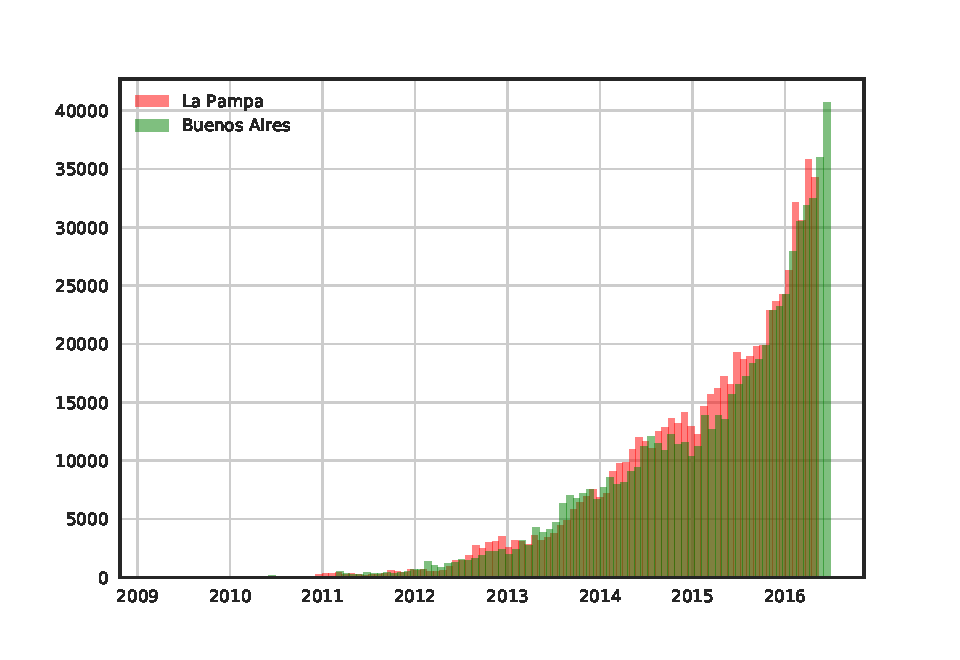
\includegraphics[width=\linewidth]{./images/histTweetsProvincia1.pdf}}
     \caption{}
     \label{fig:histTweetsProvincia1}
   \end{minipage}
   \begin {minipage}{0.49\textwidth}
     \frame{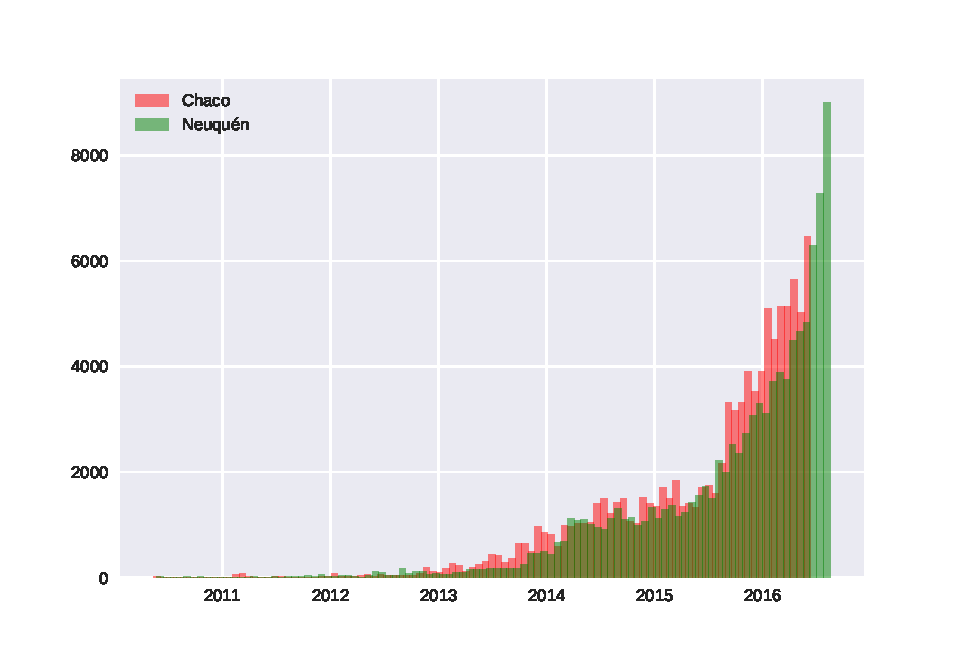
\includegraphics[width=\linewidth]{./images/histTweetsProvincia2.pdf}}
     \caption{}
     \label{fig:histTweetsProvincia2}
   \end{minipage}
   \caption { En la figura \ref{fig:histTweetsProvincia1} se presenta un histograma donde se muestra la cantidad de tweets que se hiceron por intervalo de tiempo en la provincias La Pampa y Buenos Aires. En la figura \ref{fig:histTweetsProvincia2}, se presenta el gráfico para Chaco y Neuquén.}
\end{figure}




\begin{table}[ht]
\centering

\label{tab:cantidades}
\begin{tabular}[width=0.7\textwidth]{|l|c|c|c|c|c|c|}
\hline
Provincia      & \#Palabras Distintas & \#Usuarios & \#Tweets & \#Total Palabras \\ \hline
Buenos Aires    & 191919       & 920          & 1125042    & 8974372  \\
Catamarca      & 173104       & 957          & 1057019    & 8161309   \\
Chaco          & 169476       & 964          & 976943     & 7605991   \\
Chubut         & 182592       & 954          & 1023373    & 8884745   \\
Córdoba        & 207307       & 987          & 1224266    & 10075932  \\
Corrientes     & 183292       & 939          & 1044951    & 8426940   \\
Entre Ríos      & 188679       & 969          & 1193693    & 9462986  \\
Formosa        & 169254       & 903          & 923352     & 7184382   \\
Jujuy          & 171064       & 971          & 678004     & 5951778   \\
La Pampa        & 186593       & 935          & 1085757    & 8996318  \\
La Rioja        & 186041       & 946          & 704044     & 6757277  \\
Mendoza        & 193708       & 945          & 1099717    & 9402399   \\
Misiones       & 168400       & 972          & 984218     & 7790197   \\
Neuquén        & 188038       & 927          & 1111201    & 9021449   \\
Río Negro       & 194383       & 965          & 1215361    & 9991831  \\
Salta          & 188402       & 884          & 830916     & 7506652   \\
San Juan        & 183546       & 926          & 1002322    & 8377792  \\
San Luis        & 164185       & 896          & 1006464    & 8327093  \\
Santa Cruz      & 174089       & 935          & 876621     & 7432923  \\
Santa Fe        & 201879       & 937          & 1019620    & 8862328  \\
Santiago del Estero       & 166540       & 887          & 944109     & 7355729  \\
Tierra del Fuego & 197273       & 964          & 976426     & 8559218   \\
Tucumán        & 195643       & 962          & 1093874    & 9238526 \\
  \hline
\end{tabular}
\caption{Cantidades del dataset}
\end{table}

% Tweets promedio por usuario, por provincia. (varianza)

% cantidad de tweets por usuario, cantidad media de palabras por usuario
% Ley de zipf, ver que vale con nuestro dataset

\section{Búsqueda de contrastes}

% Definir que es un contraste, que tiene un uso significativo en una region más que en otra. LAs alternativas que propusimos, z test binomial.
Diremos que una palabra tiene un contraste cuando esta tiene un uso con diferencias significativas en
distintas regiones. En este trabajo nos proponemos crear un listado con palabras con contrastes que tengan
importancia a nivel lingüistico. En este sentido, los nombres de personas, lugares, organizaciones no 
serán consideradas de interés a pesar de tener contrastes en su uso.
Este listado será ordenado por una métrica que capte en un único valor el nivel contrastivo. De esta manera, 
se seleccionará un subconjunto de palabras, de acuerdo a la métrica, las cuales serán analizadas manualmente en otros textos por la Academia Argentina de Letras.\\
El primer acercamiento para ver el contraste de las palabras lo realizamos comparando las frecuencias de las palabras 
en cada par de prinvincias de la Argentina. Para esto calculamos el cociente entre la frecuencia máxima de la palabra
en las dos provincias sobre la frecuencia mínima, al que llamaremos \textit{maxDif}. En caso de que en una de las dos provincias no se haya 
recolectado tweets con esa palabra, se tomaba en cuenta la frecuencia de la palabra con menos ocurrencias en esa provincia.
De esa manera se ordenó el listado de cada par de provincias teniendo en cuenta la división de frecuencias. \\
Sin embargo, este método imposibilitaba el trabajo manual para la Academia Argentina de Letras que debía mirar estos listados y hacer un análisis más exhaustivo sobre las palabras con mayor diferencia de frecuencias, debido a que había $\binom{23}{2} = 253$
listados (o equivalentemente 253 columnas en un mismo listado) a analizar. Además la métrica solo permitía saber si había un contraste entre dos provincias, pero no se podía tener en cuenta la frecuencia de la palabra en el resto de las provincias. 
En consecuencia las palabras se encontraban repetidas en los distintos listados y con diferentes valores de \textit{maxDif}, lo cual hacía muy díficil poder identificar en que regiones había una diferencia significativa de frecuencias. Debido a esto decidimos realizar un nuevo enfoque para encontrar las palabras con alta contrastividad en las distintas regiones, de manera que una métrica pueda reflejar el nivel de contrastividad de la palabra en un único valor.
De este modo, nos enfocamos a analizar el contraste de frecuencias de palabras sobre las provincias a través de una métrica superadora.

\subsection{Métricas para medir el contraste en la frecuencia de las palabras}
Dado que se quiere encontrar las palabras con contrastes significativos en distintas 
regiones se propone generar una métrica basada en la cantidad de información 
para poder realizar esta tarea.

Una médida que se puede usar para comparar las frecuencias de las palabras en las difentes regiones del país puede ser la entropía definida por Shannon\ref{sub:entropiaShannon}, debido a que podemos tener un valor que informe que tan uniforme es la distribución de las frecuencias de cada palabra.
Sin embargo, la entropía como única médida tiene sus desventajas. Principalmente, una palabra con una sola ocurrencia en una provincia y ninguna en las demás, tiene la entropía mínima. A pesar de que nos interesan las palabras con un contraste significativo entre regiones, dentro de ellas eligiremos las que tienne mayor cantidad de ocurrencias. Es por esto que elaboramos otra métrica que tenga en cuenta la entropía, pero que no sea la única variable a tener en cuenta.


\subsection{Valor de información}
% Describir que hace informalmente la médida de información, pondera el desorden de las palabras teniendo en cuenta sus frecuencias.
La métrica que utilizamos para ordenar los listados de palabras y detectar cuales son
las que tienen altos contrastes en su uso en distintas regiones fue inspirada sobre el
trabajo de Zanette y Montemurro \cite{montemurro2010towards}.
Ellos a diferencia de Shannon estudiaron una relación entre una médida de la información y su función semántica en el lenguaje.
A continuación detallamos el procedimiento para calcular lo que ellos llamaron
el valor de la información: \\
Dado un texto dividido en P partes iguales, se calcula la entropía  $\eta(w)$ sobre el vector de cantidad de ocurrencias en cada una de las P ventanas.
Luego se define $\widehat{\eta(w)}$  como la entropía de una permutación aleatoria del texto y promediada por todos las posibles realizaciones de la permutación de él. 
%% CHEQUEAR LA DEFINICION DE LA ENTROPIA SHUFFLEADA
Es decir, se distribuyen uniformemente las palabras en P partes y se calcula la
entropía como se hizo con el texto original. Es de esperar que en la mayoría de casos 
la entropía del texto permutado sea mayor que la médida en el calculo original. Esto 
se debe a que las palabras se distribuyen de forma más uniforme 
en las distintas partes.
Finalmente, definen al valor de la información como $I(w) = p(w) (\widehat{\eta(w)} - \eta(w))$ , con $p(w)$ la frecuencia total de la palabra en el texto. 
De esta manera se le da más importancia a las palabtas que son más frecuentes y a las palabras que tienen una baja entropía, ya que en estas el término de la diferencia es más grande.\\
Este estudio se hizo sobre tres textos, \textit{Análisis de la mente}, 
\textit{Moby Dick} y \textit{El origen de las especies} de Charles Darwin. 
En los tres libros las palabras con mayor valor de la información están 
altamente relacionadas con los temas principales.

Si bien esta métrica tiene en cuenta la frecuencia de las palabras además de la 
entropía, el texto en Twitter resulta dificil dividirlo en partes iguales. 
Esto es porque la división está pensada para dividir al texto en secciones que 
posiblemente hablen de distintos temas y nuestros textos son tweets que por lo general no superan las 10 palabras.
Otra dificultad que surge de esta métrica es la imposibilidad de realizar la media 
de todas las posibles permutaciones del texto por la limitación computacional ya que 
tenemos una cantidad muy grande de datos.

Es por eso que realizamos una métrica parecida:
Podemos pensar a las palabras del texto como una variable aleatoria W, donde cada palabra w tiene una probabilidad de aparición en una provincia dada de la Argentina. Esta probabilidad la aproximamos con la frecuencia en la que aparece, es decir la cantidad de ocurrencias de la palabra dividida por la cantidad de palabras totales.
Por otro lado sea P una variable aleatoria que cuenta la cantidad de personas que 
utilizan la palabra p en cada provincia.

Luego,
\begin{equation}
I(w) =  norm_{w}(w) * norm_{p}(w) * (\widehat{H}_{w}(w) - H_{w}(w)) * (\widehat{H}_{p}(w) - H_{p}(w))
\end{equation}

donde:
% hacer renombre de logpalabras para que quede claro que la normalización es lineal
\begin{equation}
norm_{w} = \frac{cw(w)- min(cw(w))}{max(cw(w)) - min(cw(w))}    
\end{equation}
donde $c(w)$ es igual al logaritmo sobre la cantidad de ocurrencias de esa palabra en toda la Argentina, es decir $cw(w) = log_2(cantidadOcurrencias(w))$.

Análogamente,
\begin{equation}
norm_{p} = \frac{cp(u)- min(cp(u))}{max(cp(u)) - min(cp(u))}
\end{equation}
donde $cu(u)$ es el logaritmo sobre  la cantidad de usuarios que utilizan dicha palabra en la Argentina, $c(u)= log_2(cantidadUsuarios(w)))$.


$\widehat{H}$ es la entropía con las cantidades distribuidas uniformemente y H es la entropía común.

Tanto $norm_{w}$ como $norm_{u}$ realizan una normalización del logaritmo de esas variables. Esto se debe a que el logaritmo genera una dispersión en las medidas de forma tal que su distribución sea más uniforme a lo largo de todo el rango de valores. Esto se puede ver en la figura \ref{fig:cantNorms}.
$\widehat{H}_{u}$ y $\widehat{H}_{w}$ se corresponde a las entropías de los vectores simulados de apariciones.
Esta simulación se realiza con una distribución multinomial ya que se distribuye la suma de los valores de la variable aleatoria uniformemente. 

\begin{figure}[!ht]
\centering
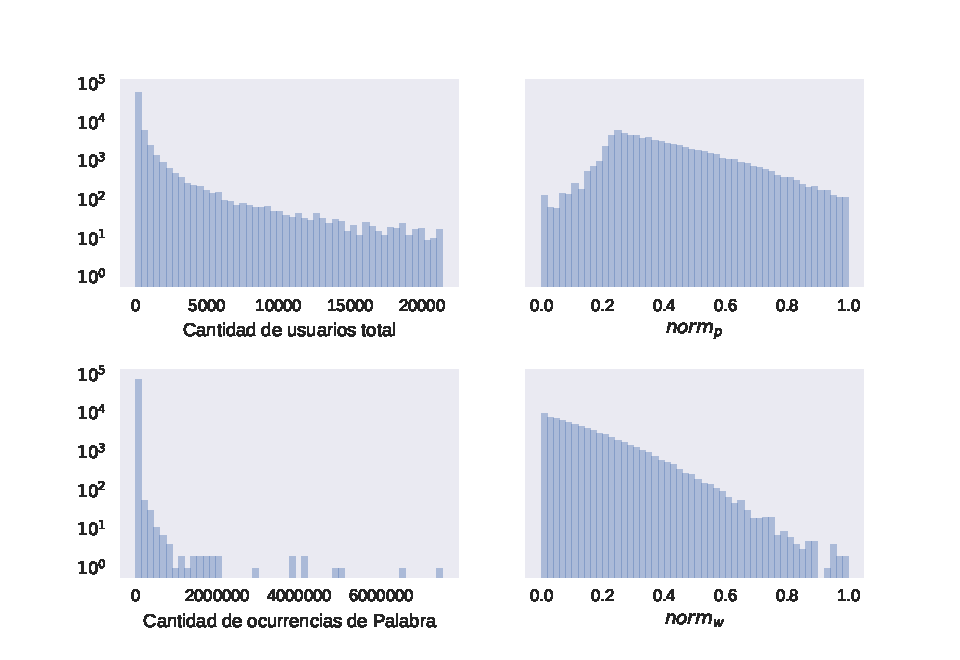
\includegraphics[width=1.0\textwidth]{./images/cantNorms.pdf}
\caption{Cantidades y sus normalizaciones} 
\label{fig:cantNorms} 
\end{figure}

El término de la diferencia de la entropía sobre la cantidad de personas que utilizan la palabra tiene como objetivo mitigar el ruido de la entropía de palabras. En particular una determinada provincia  o región pueden tener muchas ocurrencias de una palabra causado por algunos usuarios que utilizan constantemente el término. Un ejemplo de esto podrían ser bots que escriben automáticamente textos iguales (o similares) en grandes cantidades. Otra posible causa de este fenomeno podría ser la de usuarios de ciertas organizacioenes que hablan de personas, lugares o marcas de forma constante. 
Para eliminar outliers se procedió a eliminar las palabras que tenían una cantidad de usuarios menor o igual a 40 ocurrencias, como también las palabras que eran dichas por menos de 6 personas. 



% usamos la multinomial
% valor de informacion de zanette. ejemplos de como extrae las palabras más importantes/
% nos inspiramos en el valor de informacion, explicar la formula utilizada
%

\subsection{Test Hipergeométrico}


\subsection{Frecuencia de las Palabras}
\label{sub: frecuenciaPalabras}
% Ver si se hace este gráfico con todas las palabras ya que por ahora tengo el conjunto de palabras con más de 40 ocurrencias
A continuación podemos ver la distribución de la cantidad de ocurrencias de las palabras.
\begin{figure}[ht]
\centering
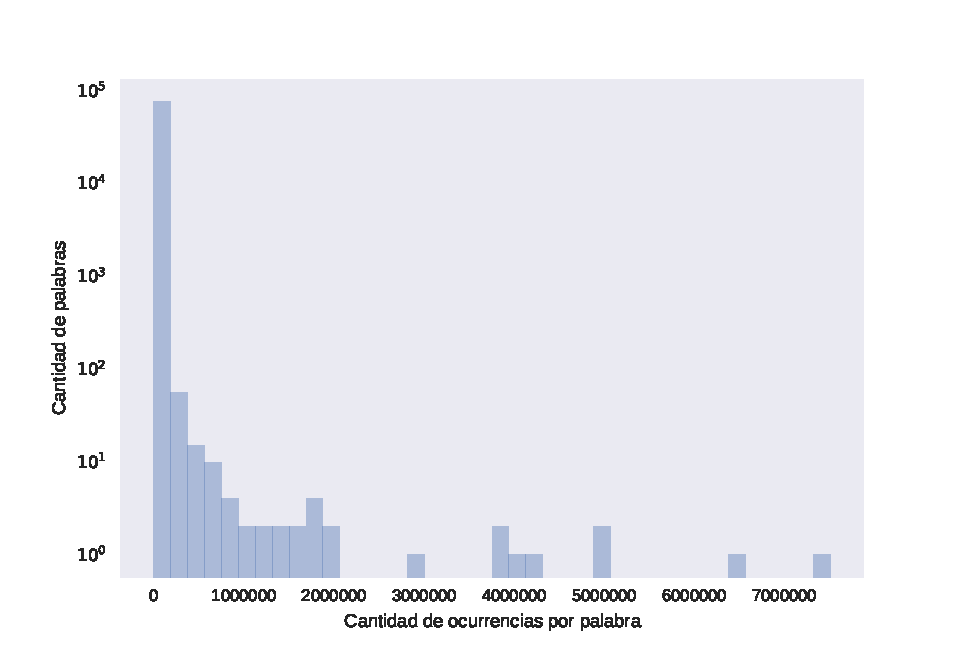
\includegraphics[width=0.8\textwidth]{./images/DistribucionOcurrenciasPalabras.pdf} 
\caption{Histograma de la cantidad de ocurrencias de las palabras} 
\label{fig:cantPalabras} 
\end{figure}

En la figura \ref{fig:cantPalabras} podemos observar que la mayoría de las palabras ocurren poco. En particular el 50\% de las palabras ocurren menos de 139 veces. Por otro lado hay pocas palabras que ocurren mucho, por ejemplo la palabra \textit{que} o la preposición \textit{de}.

\begin{table}[ht]
\centering
\label{tabla:palabrasMasOcurrentes}
\begin{tabular}{|c|c|}
\hline
Palabra & Cantidad de Ocurrencias \\ \hline
que     & 7509160                 \\
de      & 6527014                 \\
a       & 4962492                 \\
la      & 4913854                 \\
no      & 4177810                 \\
me      & 4101998                 \\
y       & 3838370                 \\
el      & 3773455                 \\
en      & 2969783                 \\
te      & 2060662                 \\
se      & 1976027                 \\
un      & 1863075                 \\
es      & 1825892                 \\
con     & 1799979                 \\
lo      & 1712189                 \\
mi      & 1643777                 \\
por     & 1553382                 \\
los     & 1498941                 \\
para    & 1398757                 \\
las     & 1212452                 \\
\hline
\end{tabular}
\caption{Cantidad de apariciones de las 20 palabras más frecuentes}

\end{table}

Si comparamos la posición de la palabra en un listado ordenado podemos ver que se cumple con la ley de Zipf. Esta es una ley empírica formulada por George Zipf en el año 1932 en la cual se establece una relación entre la frecuencia de una palabra con su posición dentro del listado de palabras ordenadas por frecuencia decreciente. En particular, sea $s$ la posición de la palabra en el listado ordenado y sea $f(s)$ la cantidad de ocurrencias de la palabra, es decir la cantidad de ocurrencias de esta dividido por el total de palabras, se puede hacer la siguiente aproximación:

$$f(s) \approx \frac{A}{s^{\alpha}}$$
donde $\alpha$ toma un valor levemente mayor a 1 y A es una constante.

\begin{figure}[ht]
\centering
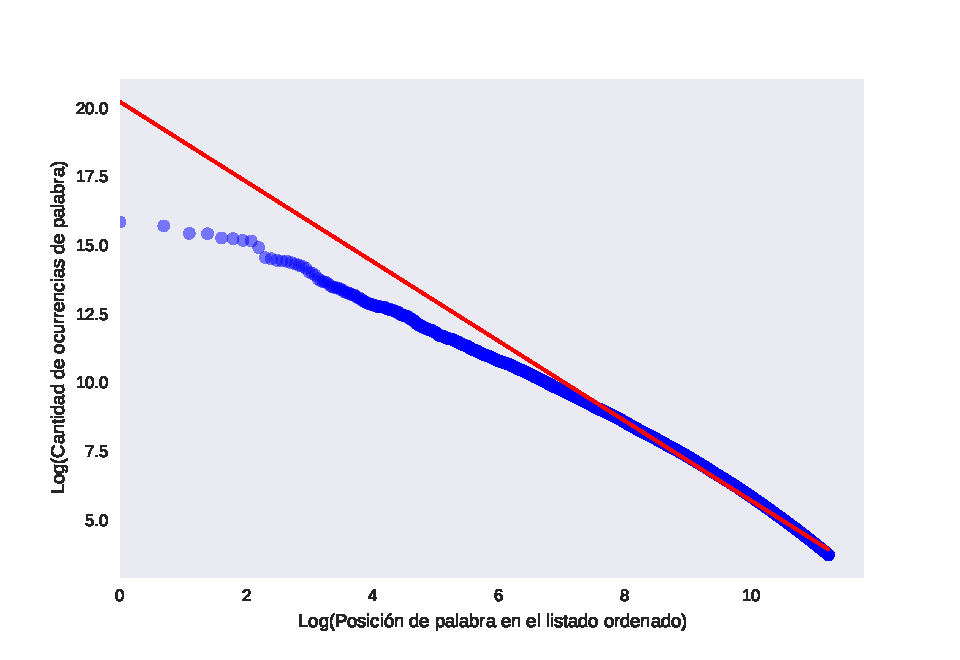
\includegraphics[width=0.8\textwidth]{./images/zipf.pdf}
\caption{Cantidad de Ocurrencias de palabra vs posición en listado ordenado. Se aplicó el logaritmo a las cantidades de ocurrencias, como también a los valores de las posiciones para mostrar la proporcionalidad entre $f(s)$ y $\frac{1}{s^{\alpha}}$} 
\label{fig:zipf} 
\end{figure}
